\documentclass[12pt,a4paper]{article}
\usepackage{geometry}
\usepackage{graphicx}
\usepackage{titlesec}
\usepackage{fancyhdr}
\usepackage{tikz}
\usetikzlibrary{shapes,arrows,positioning,calc,fit}
\usepackage{longtable}
\usepackage{booktabs}
\usepackage{enumitem}
\usepackage{hyperref}
\usepackage{ctex}
\geometry{left=3.17cm,right=3.17cm,top=2.54cm,bottom=2.54cm}

% 设置字体 - 使用系统可用字体
\setCJKmainfont{Droid Sans Fallback}
\setCJKfamilyfont{songti}{AR PL UMing CN}[AutoFakeBold]

% 设置超链接样式
\hypersetup{
colorlinks=true,
linkcolor=blue,
filecolor=magenta,      
urlcolor=cyan,
citecolor=blue,
}

% 设置页眉高度
\setlength{\headheight}{15pt}

% 页眉页脚设置
\pagestyle{fancy}
\fancyhf{}
\fancyhead[C]{智记便签软件设计规格说明书}
\fancyfoot[C]{\thepage}

% 标题格式
\titleformat{\section}{\Large\bfseries}{\thesection}{1em}{}
\titleformat{\subsection}{\large\bfseries}{\thesubsection}{1em}{}
\titleformat{\subsubsection}{\normalsize\bfseries}{\thesubsubsection}{1em}{}

\begin{document}

\begin{titlepage}
\centering

% 顶部空白
\vspace*{3cm}

% --- 2号宋体 (22pt) ---
{\CJKfamily{songti}\fontsize{22}{26}\selectfont 计算机科学与技术学院}\\[2cm]

% --- 小1号黑体 (24pt), 粗体 ---
{\fontsize{24}{28}\selectfont\bfseries 智记便签 项目}\\[1cm]
{\fontsize{24}{28}\selectfont\bfseries 软件设计规格说明}\\[4cm]

% --- 4号宋体 (14pt) ---
\begin{center}
{\CJKfamily{songti}\fontsize{14}{18}\selectfont
\begin{tabular}{l@{\hspace{1cm}}l}
% --- 第一位学生 ---
\makebox[4cm][s]{学 号:} & \makebox[8cm][l]{2023064128} \\[1.2cm]
\makebox[4cm][s]{专 业:} & \makebox[8cm][l]{计算机科学与技术} \\[1.2cm]
\makebox[4cm][s]{学生姓名:} & \makebox[8cm][l]{潘铮} \\[1.2cm]

% --- 间隔 ---
\\[0.5cm] 

% --- 第二位学生 ---
\makebox[4cm][s]{学 号:} & \makebox[8cm][l]{2023064129} \\[1.2cm]
\makebox[4cm][s]{专 业:} & \makebox[8cm][l]{计算机科学与技术} \\[1.2cm]
\makebox[4cm][s]{学生姓名:} & \makebox[8cm][l]{季凯阳} \\[1.2cm]

% --- 其他信息 ---
\makebox[4cm][s]{人员分工:} & \makebox[8cm][l]{} \\[1.2cm]
\makebox[4cm][s]{合作方法:} & \makebox[8cm][l]{} \\[2cm]
\makebox[4cm][s]{任课教师:} & \makebox[8cm][l]{郑丽颖 教授} \\
\end{tabular}
}
\end{center}

\vfill

\end{titlepage}

\newpage
\tableofcontents
\newpage

\section{引言}

\subsection{编写目的}

本文档是智记便签(Smart Note)项目的软件设计规格说明书(Software Design Specification, SDD),旨在详细描述系统的架构设计、模块设计、接口设计和数据库设计。本文档基于已完成的软件需求规格说明书(SRS),为开发人员提供详细的设计方案和实现指导。

本文档的预期读者包括:
\begin{itemize}[leftmargin=2cm]
\item 项目开发人员:作为编码实现的依据
\item 测试人员:作为测试用例设计的参考
\item 项目管理人员:用于进度跟踪和质量评估
\item 维护人员:作为系统维护和升级的参考文档
\end{itemize}

\subsection{项目背景}

\textbf{项目名称}:智记便签(Smart Note)

\textbf{项目背景}:智记便签是在小米便签基础上进行功能增强和优化的移动端便签应用。本项目新增Markdown富文本支持和增强的导出分享功能,为用户提供更加专业和高效的笔记体验。

\subsection{定义、首字母缩写词和缩略语}

\begin{longtable}{|p{3cm}|p{10cm}|}
\hline
\textbf{术语} & \textbf{定义} \\
\hline
SDD & Software Design Description,软件设计规格说明 \\
\hline
SRS & Software Requirements Specification,软件需求规格说明 \\
\hline
MVC & Model-View-Controller,模型-视图-控制器架构模式 \\
\hline
DAO & Data Access Object,数据访问对象 \\
\hline
UML & Unified Modeling Language,统一建模语言 \\
\hline
API & Application Programming Interface,应用程序编程接口 \\
\hline
UI & User Interface,用户界面 \\
\hline
Markdown & 一种轻量级标记语言 \\
\hline
ContentProvider & Android平台的数据共享机制 \\
\hline
SQLite & 轻量级关系型数据库管理系统 \\
\hline
\end{longtable}

\subsection{参考资料}

\begin{enumerate}[leftmargin=2cm]
\item 智记便签软件需求规格说明书(SRS\_智记便签.tex)
\item GB/T 8567-2006 计算机软件文档编制规范
\item Android开发者文档:https://developer.android.com/
\item 小米便签(MiCode Notes)开源项目:https://github.com/MiCode/Notes
\item 《软件工程:实践者的研究方法》(第8版)
\end{enumerate}

\section{系统架构设计}

\subsection{系统总体架构}

智记便签采用经典的Android应用三层架构设计,将系统分为表示层(Presentation Layer)、业务逻辑层(Business Logic Layer)和数据访问层(Data Access Layer)。\hyperref[fig:system_architecture]{图\ref{fig:system_architecture}}展示了系统的总体架构。

\begin{figure}[h]
\centering
\begin{tikzpicture}[scale=0.85, transform shape]
% 表示层
\node[draw, rectangle, minimum width=12cm, minimum height=2cm, align=center] (ui) at (0,0) 
{\textbf{表示层 (Presentation Layer)} \\ NotesListActivity, NoteEditActivity, Widget};

% 业务逻辑层
\node[draw, rectangle, minimum width=12cm, minimum height=2cm, align=center, below of=ui, yshift=-2cm] (business) 
{\textbf{业务逻辑层 (Business Logic Layer)} \\ WorkingNote, MarkdownRenderer, FormatConverter, ShareHelper};

% 数据访问层
\node[draw, rectangle, minimum width=12cm, minimum height=2cm, align=center, below of=business, yshift=-2cm] (data) 
{\textbf{数据访问层 (Data Access Layer)} \\ NotesProvider, NotesDatabaseHelper};

% 数据存储层
\node[draw, rectangle, minimum width=12cm, minimum height=1.5cm, align=center, below of=data, yshift=-1.8cm] (storage) 
{\textbf{数据存储层} \\ SQLite Database};

% 外部服务
\node[draw, rectangle, minimum width=5cm, minimum height=1.5cm, align=center, right of=data, xshift=9cm] (external) 
{\textbf{外部服务} \\ Google Tasks API};

% 连接线
\draw[<->, thick] (ui) -- (business);
\draw[<->, thick] (business) -- (data);
\draw[<->, thick] (data) -- (storage);
\draw[<->, thick] (data) -- (external);
\end{tikzpicture}
\caption{系统总体架构图}
\label{fig:system_architecture}
\end{figure}

\subsection{架构层次说明}

\subsubsection{表示层(Presentation Layer)}

表示层负责与用户的交互,包括显示界面和接收用户输入。主要组件包括:

\begin{itemize}[leftmargin=2cm]
\item \textbf{NotesListActivity}:显示便签列表,提供便签的浏览、搜索和分类功能
\item \textbf{NoteEditActivity}:便签编辑界面,支持文本输入、Markdown编辑和预览
\item \textbf{AlarmAlertActivity}:提醒通知界面
\item \textbf{NoteWidget}:桌面小部件,提供快速访问和编辑功能
\item \textbf{FormatDialog}:导出格式选择对话框
\end{itemize}

\subsubsection{业务逻辑层(Business Logic Layer)}

业务逻辑层处理应用的核心功能和业务规则。主要组件包括:

\begin{itemize}[leftmargin=2cm]
\item \textbf{WorkingNote}:便签的业务模型,封装便签的操作逻辑
\item \textbf{MarkdownRenderer}:Markdown渲染引擎,将Markdown文本转换为格式化显示
\item \textbf{FormatConverter}:格式转换器,支持将便签转换为多种导出格式
\item \textbf{ShareHelper}:分享助手,处理便签的分享逻辑
\item \textbf{SyncManager}:同步管理器,处理云同步逻辑
\end{itemize}

\subsubsection{数据访问层(Data Access Layer)}

数据访问层提供统一的数据访问接口,封装数据库操作细节。主要组件包括:

\begin{itemize}[leftmargin=2cm]
\item \textbf{NotesProvider}:ContentProvider实现,提供标准化的数据访问接口
\item \textbf{NotesDatabaseHelper}:数据库助手类,管理数据库创建和版本升级
\end{itemize}

\subsection{设计模式应用}

系统采用多种设计模式以提高代码质量和可维护性:

\begin{itemize}[leftmargin=2cm]
\item \textbf{MVC模式}:整体架构采用MVC模式,分离界面、逻辑和数据
\item \textbf{单例模式}:MarkdownRenderer、SyncManager等工具类采用单例模式
\item \textbf{工厂模式}:FormatConverter使用工厂模式创建不同格式的转换器
\item \textbf{观察者模式}:数据变化时使用ContentObserver通知UI更新
\item \textbf{策略模式}:不同的导出格式使用不同的转换策略
\end{itemize}

\section{模块详细设计}

\subsection{便签编辑模块}

\subsubsection{模块概述}

便签编辑模块是系统的核心模块,负责便签的创建、编辑、保存和显示。该模块新增了Markdown编辑和预览功能。

\subsubsection{类设计}

\hyperref[fig:edit_module_class]{图\ref{fig:edit_module_class}}展示了便签编辑模块的类图。

\begin{figure}[h]
\centering
\begin{tikzpicture}[scale=0.7, transform shape]
% NoteEditActivity类
\node[draw, rectangle, minimum width=5.5cm, align=left] (activity) at (0,0) {
\textbf{NoteEditActivity} \\
\rule{5.5cm}{0.4pt} \\
-mWorkingNote: WorkingNote \\
-mNoteEditor: EditText \\
-mPreviewView: TextView \\
-mPreviewButton: Button \\
-mIsPreviewMode: boolean \\
-mMarkdownRenderer: MarkdownRenderer \\
\rule{5.5cm}{0.4pt} \\
+onCreate(): void \\
+togglePreview(): void \\
+renderMarkdown(): void \\
+switchToEditMode(): void \\
+switchToPreviewMode(): void \\
+saveNote(): void \\
+shareNote(): void
};

% WorkingNote类
\node[draw, rectangle, minimum width=5cm, align=left, right of=activity, xshift=8cm] (working) {
\textbf{WorkingNote} \\
\rule{5cm}{0.4pt} \\
-mNoteId: long \\
-mContent: String \\
-mModifiedDate: long \\
-mAlertDate: long \\
-mFolderId: long \\
\rule{5cm}{0.4pt} \\
+loadNote(id: long): void \\
+saveNote(): boolean \\
+setContent(content: String): void \\
+getContent(): String \\
+setAlertDate(date: long): void \\
+markDeleted(): void
};

% MarkdownRenderer类
\node[draw, rectangle, minimum width=5cm, align=left, below of=activity, yshift=-6cm] (renderer) {
\textbf{MarkdownRenderer} \\
\rule{5cm}{0.4pt} \\
-markwon: Markwon \\
-context: Context \\
-instance: MarkdownRenderer \\
\rule{5cm}{0.4pt} \\
+getInstance(ctx: Context): MarkdownRenderer \\
+render(text: String): Spanned \\
+setMarkdown(tv: TextView, text: String): void \\
-initialize(): void
};

% 关联
\draw[->] (activity) -- node[above, font=\small] {使用} (working);
\draw[->] (activity) -- node[right, font=\small] {使用} (renderer);
\end{tikzpicture}
\caption{便签编辑模块类图}
\label{fig:edit_module_class}
\end{figure}

\subsubsection{主要接口}

\textbf{NoteEditActivity主要接口}:

\begin{itemize}[leftmargin=2cm]
\item \textbf{togglePreview()}: void
\begin{itemize}
\item 功能:切换编辑模式和预览模式
\item 前置条件:Activity已初始化
\item 后置条件:界面切换到相应模式
\end{itemize}

\item \textbf{renderMarkdown()}: void
\begin{itemize}
\item 功能:渲染Markdown文本为格式化显示
\item 前置条件:存在待渲染的Markdown文本
\item 后置条件:预览视图显示渲染结果
\end{itemize}

\item \textbf{saveNote()}: void
\begin{itemize}
\item 功能:保存当前便签到数据库
\item 前置条件:WorkingNote已初始化
\item 后置条件:便签内容保存成功
\end{itemize}
\end{itemize}

\textbf{MarkdownRenderer主要接口}:

\begin{itemize}[leftmargin=2cm]
\item \textbf{getInstance(Context)}: MarkdownRenderer
\begin{itemize}
\item 功能:获取MarkdownRenderer单例实例
\item 参数:Context - Android上下文
\item 返回:MarkdownRenderer实例
\end{itemize}

\item \textbf{render(String)}: Spanned
\begin{itemize}
\item 功能:将Markdown文本渲染为Spanned对象
\item 参数:text - Markdown格式文本
\item 返回:渲染后的Spanned对象
\end{itemize}
\end{itemize}

\subsubsection{算法设计}

\textbf{Markdown预览切换算法}:

\begin{enumerate}[leftmargin=2cm]
\item 检查当前模式(编辑/预览)
\item 如果当前为编辑模式:
\begin{enumerate}
\item 获取EditText中的文本内容
\item 调用MarkdownRenderer.render()渲染文本
\item 将渲染结果设置到TextView
\item 隐藏EditText,显示TextView
\item 更新按钮文本为"编辑"
\end{enumerate}
\item 如果当前为预览模式:
\begin{enumerate}
\item 隐藏TextView,显示EditText
\item 更新按钮文本为"预览"
\end{enumerate}
\end{enumerate}

\subsection{导出分享模块}

\subsubsection{模块概述}

导出分享模块支持将便签导出为多种格式(纯文本、Markdown、HTML)并通过系统分享功能发送。

\subsubsection{类设计}

\hyperref[fig:share_module_class]{图\ref{fig:share_module_class}}展示了导出分享模块的类图。

\begin{figure}[h]
\centering
\begin{tikzpicture}[scale=0.65, transform shape]
% FormatConverter类
\node[draw, rectangle, minimum width=6cm, align=left] (converter) at (0,4) {
\textbf{FormatConverter} \\
\rule{6cm}{0.4pt} \\
\rule{6cm}{0.4pt} \\
+convertToPlainText(text: String): String \\
+convertToMarkdown(text: String): String \\
+convertToHtml(text: String): String \\
-addCssStyles(html: String): String \\
-renderMarkdownToHtml(md: String): String
};

% ShareHelper类
\node[draw, rectangle, minimum width=6cm, below of=converter, yshift=-5cm, align=left] (helper) {
\textbf{ShareHelper} \\
\rule{6cm}{0.4pt} \\
-context: Context \\
-converter: FormatConverter \\
\rule{6cm}{0.4pt} \\
+shareContent(content: String, format: Format): void \\
+createShareIntent(content: String, format: Format): Intent \\
-getMimeType(format: Format): String
};

% FormatDialog类
\node[draw, rectangle, minimum width=6cm, right of=converter, xshift=8.5cm, align=left] (dialog) {
\textbf{FormatDialog} \\
\rule{6cm}{0.4pt} \\
-listener: OnFormatSelectedListener \\
-formats: List<Format> \\
\rule{6cm}{0.4pt} \\
+show(context: Context): void \\
+setOnFormatSelectedListener(listener): void \\
+dismiss(): void \\
-buildDialog(): AlertDialog
};

% Format枚举
\node[draw, rectangle, minimum width=6cm, below of=dialog, yshift=-4.5cm, align=left] (format) {
\textbf{<<enumeration>> Format} \\
\rule{6cm}{0.4pt} \\
PLAIN\_TEXT \\
MARKDOWN \\
HTML \\
\rule{6cm}{0.4pt} \\
+getDisplayName(): String \\
+getMimeType(): String
};

% 关联
\draw[->] (dialog) -- node[above, font=\small] {使用} (converter);
\draw[->] (helper) -- node[right, font=\small] {依赖} (converter);
\draw[->] (dialog) -- node[right, font=\small] {使用} (format);
\draw[->] (helper) -- node[above, font=\small] {使用} (format);
\end{tikzpicture}
\caption{导出分享模块类图}
\label{fig:share_module_class}
\end{figure}

\subsubsection{主要接口}

\textbf{FormatConverter主要接口}:

\begin{itemize}[leftmargin=2cm]
\item \textbf{convertToPlainText(String)}: String
\begin{itemize}
\item 功能:转换为纯文本格式
\item 参数:text - 原始文本
\item 返回:纯文本内容
\end{itemize}

\item \textbf{convertToHtml(String)}: String
\begin{itemize}
\item 功能:转换为HTML格式
\item 参数:text - Markdown文本
\item 返回:包含CSS样式的完整HTML文档
\end{itemize}
\end{itemize}

\textbf{ShareHelper主要接口}:

\begin{itemize}[leftmargin=2cm]
\item \textbf{shareContent(String, Format)}: void
\begin{itemize}
\item 功能:分享内容到其他应用
\item 参数:content - 内容文本, format - 导出格式
\item 后置条件:启动系统分享界面
\end{itemize}
\end{itemize}

\subsubsection{算法设计}

\textbf{HTML格式转换算法}:

\begin{enumerate}[leftmargin=2cm]
\item 检查文本是否为Markdown格式
\item 使用MarkdownRenderer将Markdown渲染为HTML
\item 创建完整的HTML文档结构
\item 添加CSS样式:
\begin{enumerate}
\item 设置字体、字号、行距
\item 定义标题样式
\item 定义列表样式
\item 定义代码块样式
\end{enumerate}
\item 返回完整HTML文档
\end{enumerate}

\subsection{数据管理模块}

\subsubsection{模块概述}

数据管理模块负责所有数据的持久化存储和访问,通过ContentProvider提供统一的数据访问接口。

\subsubsection{类设计}

\hyperref[fig:data_module_class]{图\ref{fig:data_module_class}}展示了数据管理模块的类图。

\begin{figure}[h]
\centering
\begin{tikzpicture}[scale=0.65, transform shape]
% NotesProvider类
\node[draw, rectangle, minimum width=6.5cm, align=left] (provider) at (0,0) {
\textbf{NotesProvider extends ContentProvider} \\
\rule{6.5cm}{0.4pt} \\
-mHelper: NotesDatabaseHelper \\
\rule{6.5cm}{0.4pt} \\
+onCreate(): boolean \\
+query(uri, projection, selection, ...): Cursor \\
+insert(uri, values): Uri \\
+update(uri, values, selection, ...): int \\
+delete(uri, selection, ...): int \\
+getType(uri): String
};

% NotesDatabaseHelper类
\node[draw, rectangle, minimum width=6.5cm, align=left, below of=provider, yshift=-6.5cm] (helper) {
\textbf{NotesDatabaseHelper extends SQLiteOpenHelper} \\
\rule{6.5cm}{0.4pt} \\
-DATABASE\_NAME: String \\
-DATABASE\_VERSION: int \\
\rule{6.5cm}{0.4pt} \\
+onCreate(db: SQLiteDatabase): void \\
+onUpgrade(db, oldVersion, newVersion): void \\
+createNotesTable(db: SQLiteDatabase): void \\
+createDataTable(db: SQLiteDatabase): void
};

% Note类
\node[draw, rectangle, minimum width=5.5cm, align=left, right of=provider, xshift=9cm, yshift=0.5cm] (note) {
\textbf{Note} \\
\rule{5.5cm}{0.4pt} \\
+ID: String \\
+TYPE: String \\
+CREATED\_DATE: String \\
+MODIFIED\_DATE: String \\
+ALERT\_DATE: String \\
+PARENT\_ID: String \\
+SYNC\_ID: String \\
\rule{5.5cm}{0.4pt} \\
// 常量定义
};

% NoteData类
\node[draw, rectangle, minimum width=5.5cm, align=left, below of=note, yshift=-4.5cm] (data) {
\textbf{NoteData} \\
\rule{5.5cm}{0.4pt} \\
+ID: String \\
+MIME\_TYPE: String \\
+NOTE\_ID: String \\
+CONTENT: String \\
+DATA1: String \\
+DATA2: String \\
\rule{5.5cm}{0.4pt} \\
// 常量定义
};

% 关联
\draw[->] (provider) -- node[right, font=\small] {使用} (helper);
\draw[dashed, ->] (provider) -- node[above, font=\small] {定义} (note);
\draw[dashed, ->] (provider) -- node[above, font=\small] {定义} (data);
\end{tikzpicture}
\caption{数据管理模块类图}
\label{fig:data_module_class}
\end{figure}

\subsubsection{主要接口}

\textbf{NotesProvider主要接口}:

\begin{itemize}[leftmargin=2cm]
\item \textbf{query(Uri, String[], String, String[], String)}: Cursor
\begin{itemize}
\item 功能:查询数据库数据
\item 参数:uri - 查询URI, projection - 查询列, selection - WHERE子句
\item 返回:查询结果Cursor
\end{itemize}

\item \textbf{insert(Uri, ContentValues)}: Uri
\begin{itemize}
\item 功能:插入新数据
\item 参数:uri - 插入URI, values - 数据值
\item 返回:新插入数据的URI
\end{itemize}

\item \textbf{update(Uri, ContentValues, String, String[])}: int
\begin{itemize}
\item 功能:更新数据
\item 参数:uri - 更新URI, values - 新数据值, selection - WHERE子句
\item 返回:受影响的行数
\end{itemize}
\end{itemize}

\section{数据库设计}

\subsection{数据库概要}

智记便签使用SQLite数据库进行本地数据存储。数据库名称为notes.db,当前版本为3。数据库包含两个核心数据表:note表和data表。

\subsection{数据表设计}

\subsubsection{note表}

note表存储便签的元数据信息。表结构如下:

\begin{longtable}{|p{3.5cm}|p{2cm}|p{2cm}|p{5.5cm}|}
\hline
\textbf{字段名} & \textbf{类型} & \textbf{约束} & \textbf{说明} \\
\hline
\endfirsthead
\hline
\textbf{字段名} & \textbf{类型} & \textbf{约束} & \textbf{说明} \\
\hline
\endhead
\_id & INTEGER & PRIMARY KEY & 便签唯一标识符,自增 \\
\hline
type & INTEGER & NOT NULL & 便签类型(0=普通便签, 1=文件夹) \\
\hline
created\_date & INTEGER & NOT NULL & 创建时间(Unix时间戳,毫秒) \\
\hline
modified\_date & INTEGER & NOT NULL & 最后修改时间(Unix时间戳,毫秒) \\
\hline
sync\_id & INTEGER & & 云同步ID,与Google Tasks关联 \\
\hline
parent\_id & INTEGER & DEFAULT 0 & 父文件夹ID,0表示根目录 \\
\hline
alerted\_date & INTEGER & & 提醒时间(Unix时间戳,毫秒) \\
\hline
widget\_id & INTEGER & & 关联的桌面小部件ID \\
\hline
widget\_type & INTEGER & & 小部件类型 \\
\hline
bg\_color\_id & INTEGER & & 背景颜色ID \\
\hline
has\_attachment & INTEGER & DEFAULT 0 & 是否有附件(预留字段) \\
\hline
notes\_count & INTEGER & DEFAULT 0 & 文件夹包含的便签数量 \\
\hline
version & INTEGER & DEFAULT 0 & 版本号,用于同步冲突解决 \\
\hline
\end{longtable}

\subsubsection{data表}

data表存储便签的具体内容数据。表结构如下:

\begin{longtable}{|p{3.5cm}|p{2cm}|p{2cm}|p{5.5cm}|}
\hline
\textbf{字段名} & \textbf{类型} & \textbf{约束} & \textbf{说明} \\
\hline
\endfirsthead
\hline
\textbf{字段名} & \textbf{类型} & \textbf{约束} & \textbf{说明} \\
\hline
\endhead
\_id & INTEGER & PRIMARY KEY & 数据唯一标识符,自增 \\
\hline
mime\_type & TEXT & NOT NULL & 数据MIME类型(如text/note) \\
\hline
note\_id & INTEGER & NOT NULL & 关联的便签ID(外键) \\
\hline
content & TEXT & NOT NULL & 实际内容(Markdown原文) \\
\hline
data1 & INTEGER & & 扩展字段1(如联系人ID) \\
\hline
data2 & INTEGER & & 扩展字段2 \\
\hline
data3 & TEXT & & 扩展字段3(如联系人姓名) \\
\hline
data4 & TEXT & & 扩展字段4 \\
\hline
data5 & TEXT & & 扩展字段5 \\
\hline
\end{longtable}

\subsection{数据库关系图}

\hyperref[fig:er_diagram]{图\ref{fig:er_diagram}}展示了数据库的实体关系图。

\begin{figure}[h]
\centering
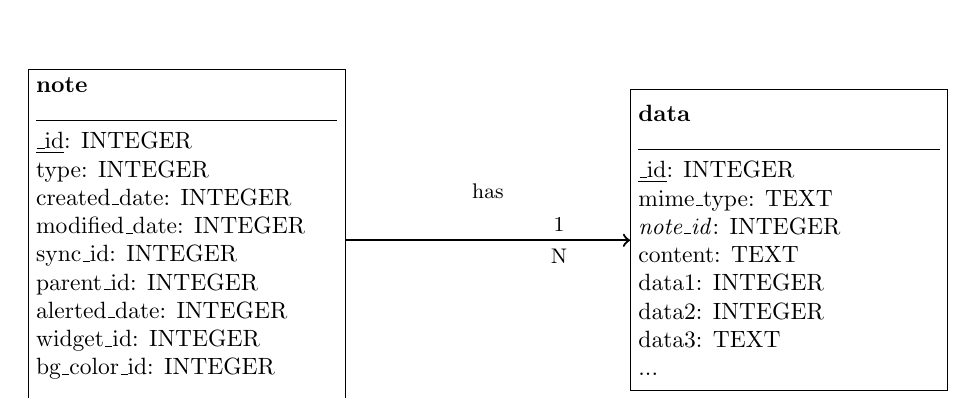
\begin{tikzpicture}[scale=0.85, transform shape]
% note表
\node[draw, rectangle, minimum width=4.5cm, minimum height=5cm, align=left] (note) at (0,0) {
\textbf{note} \\
\rule{4.5cm}{0.4pt} \\
\underline{\_id}: INTEGER \\
type: INTEGER \\
created\_date: INTEGER \\
modified\_date: INTEGER \\
sync\_id: INTEGER \\
parent\_id: INTEGER \\
alerted\_date: INTEGER \\
widget\_id: INTEGER \\
bg\_color\_id: INTEGER \\
...
};

% data表
\node[draw, rectangle, minimum width=4.5cm, minimum height=4.5cm, align=left, right of=note, xshift=8cm] (data) {
\textbf{data} \\
\rule{4.5cm}{0.4pt} \\
\underline{\_id}: INTEGER \\
mime\_type: TEXT \\
\textit{note\_id}: INTEGER \\
content: TEXT \\
data1: INTEGER \\
data2: INTEGER \\
data3: TEXT \\
...
};

% 关系
\draw[-, thick] (note.east) -- (4.5,0) -- (4.5,0);
\draw[->, thick] (4.5,0) -- (data.west) node[midway, above, font=\small] {1} node[midway, below, font=\small] {N};
\node[above, font=\small] at (4.5,0.5) {has};
\end{tikzpicture}
\caption{数据库实体关系图}
\label{fig:er_diagram}
\end{figure}

\subsection{索引设计}

为提高查询性能,在以下字段上建立索引:

\begin{itemize}[leftmargin=2cm]
\item \textbf{note表}:
\begin{itemize}
\item parent\_id索引:加速按文件夹查询便签
\item modified\_date索引:加速按修改时间排序
\item alerted\_date索引:加速查询待提醒的便签
\end{itemize}
\item \textbf{data表}:
\begin{itemize}
\item note\_id索引:加速根据便签ID查询内容
\item mime\_type索引:加速按类型查询数据
\end{itemize}
\end{itemize}

\subsection{数据完整性约束}

\begin{itemize}[leftmargin=2cm]
\item \textbf{主键约束}:\_id字段为主键,确保唯一性
\item \textbf{外键约束}:data表的note\_id引用note表的\_id,级联删除
\item \textbf{非空约束}:关键字段(type, created\_date, modified\_date, content等)不允许为空
\item \textbf{默认值约束}:parent\_id默认为0,has\_attachment默认为0
\end{itemize}

\section{接口设计}

\subsection{外部接口}

\subsubsection{ContentProvider接口}

NotesProvider实现了标准的ContentProvider接口,供外部应用或组件访问便签数据。

\textbf{URI定义}:

\begin{longtable}{|p{5cm}|p{8cm}|}
\hline
\textbf{URI} & \textbf{说明} \\
\hline
content://com.xiaomi.notes/note & 访问所有便签 \\
\hline
content://com.xiaomi.notes/note/\# & 访问特定ID的便签 \\
\hline
content://com.xiaomi.notes/data & 访问所有数据 \\
\hline
content://com.xiaomi.notes/data/\# & 访问特定ID的数据 \\
\hline
content://com.xiaomi.notes/note/\#/data & 访问特定便签的所有数据 \\
\hline
\end{longtable}

\textbf{MIME类型}:

\begin{itemize}[leftmargin=2cm]
\item vnd.android.cursor.dir/note:便签集合
\item vnd.android.cursor.item/note:单个便签
\item vnd.android.cursor.dir/data:数据集合
\item vnd.android.cursor.item/data:单条数据
\end{itemize}

\subsubsection{Intent接口}

\textbf{分享Intent}:

\begin{itemize}[leftmargin=2cm]
\item Action: ACTION\_SEND
\item Type: 根据导出格式确定(text/plain, text/markdown, text/html)
\item Extra: EXTRA\_TEXT(内容), EXTRA\_SUBJECT(标题)
\end{itemize}

\subsection{内部接口}

\subsubsection{模块间接口}

\textbf{表示层 → 业务逻辑层}:

\begin{itemize}[leftmargin=2cm]
\item WorkingNote.loadNote(long noteId):加载便签
\item WorkingNote.saveNote():保存便签
\item MarkdownRenderer.render(String text):渲染Markdown
\item FormatConverter.convertToHtml(String text):转换为HTML
\end{itemize}

\textbf{业务逻辑层 → 数据访问层}:

\begin{itemize}[leftmargin=2cm]
\item ContentResolver.query(...):查询数据
\item ContentResolver.insert(...):插入数据
\item ContentResolver.update(...):更新数据
\item ContentResolver.delete(...):删除数据
\end{itemize}

\section{用户界面设计}

\subsection{界面结构}

\hyperref[fig:ui_structure]{图\ref{fig:ui_structure}}展示了应用的界面导航结构。

\begin{figure}[h]
\centering
\begin{tikzpicture}[scale=0.8, transform shape]
% 主界面
\node[draw, rectangle, minimum width=4cm, minimum height=1.2cm] (list) at (0,0) {便签列表界面};

% 编辑界面
\node[draw, rectangle, minimum width=4cm, minimum height=1.2cm, below of=list, xshift=-5cm, yshift=-1.5cm] (edit) {便签编辑界面};

% 预览模式
\node[draw, rectangle, minimum width=4cm, minimum height=1.2cm, below of=edit, yshift=-1.5cm] (preview) {Markdown预览};

% 分享对话框
\node[draw, rectangle, minimum width=4cm, minimum height=1.2cm, right of=edit, xshift=5cm] (share) {格式选择对话框};

% 搜索界面
\node[draw, rectangle, minimum width=4cm, minimum height=1.2cm, below of=list, xshift=5cm, yshift=-1.5cm] (search) {搜索界面};

% 连接线
\draw[->, thick] (list) -- node[left, font=\small] {打开便签} (edit);
\draw[->, thick] (list) -- node[right, font=\small] {搜索} (search);
\draw[<->, thick] (edit) -- node[right, font=\small] {切换} (preview);
\draw[->, thick] (edit) -- node[above, font=\small] {分享} (share);
\end{tikzpicture}
\caption{用户界面导航结构图}
\label{fig:ui_structure}
\end{figure}

\subsection{便签列表界面}

\textbf{界面组成}:

\begin{itemize}[leftmargin=2cm]
\item 标题栏:显示应用名称"智记便签",包含搜索图标
\item 便签列表:ListView或RecyclerView显示便签,支持滑动
\item 浮动按钮:右下角的"+"按钮,用于创建新便签
\item 侧边栏(可选):显示文件夹列表
\end{itemize}

\textbf{列表项设计}:

\begin{itemize}[leftmargin=2cm]
\item 第一行:便签标题或首行内容(粗体)
\item 第二行:便签预览内容(灰色,最多显示2行)
\item 第三行:修改时间、提醒图标(如有)
\item 左侧:背景颜色标识条
\end{itemize}

\subsection{便签编辑界面}

\textbf{编辑模式布局}:

\begin{itemize}[leftmargin=2cm]
\item 标题栏:返回按钮、便签标题(可编辑)、菜单按钮
\item 编辑区域:全屏EditText,支持多行文本输入
\item 底部工具栏:
\begin{itemize}
\item 预览按钮:切换到预览模式
\item 分享按钮:打开分享对话框
\item 提醒按钮:设置提醒时间
\item 更多按钮:其他操作(删除、移动等)
\end{itemize}
\end{itemize}

\textbf{预览模式布局}:

\begin{itemize}[leftmargin=2cm]
\item 标题栏:同编辑模式
\item 预览区域:TextView显示渲染后的Markdown内容
\item 底部工具栏:编辑按钮(返回编辑模式)、分享按钮
\end{itemize}

\subsection{格式选择对话框}

\textbf{对话框设计}:

\begin{itemize}[leftmargin=2cm]
\item 标题:"选择导出格式"
\item 选项列表:
\begin{itemize}
\item 纯文本(说明:移除所有格式标记)
\item Markdown(说明:保持原始Markdown格式)
\item HTML(说明:转换为网页格式)
\end{itemize}
\item 底部按钮:取消、确定
\end{itemize}

\section{非功能性设计}

\subsection{性能设计}

\subsubsection{响应时间优化}

\begin{itemize}[leftmargin=2cm]
\item \textbf{异步加载}:使用AsyncQueryHandler进行数据库查询,避免阻塞UI线程
\item \textbf{懒加载}:列表采用分页加载,每次加载20-30条便签
\item \textbf{缓存策略}:Markdown渲染结果缓存,避免重复渲染
\item \textbf{索引优化}:在常用查询字段上建立索引,提高查询速度
\end{itemize}

\subsubsection{内存优化}

\begin{itemize}[leftmargin=2cm]
\item \textbf{及时释放}:使用完Cursor后及时关闭,避免内存泄漏
\item \textbf{对象池}:频繁创建的对象使用对象池技术
\item \textbf{图片压缩}:如果支持图片附件,需进行适当压缩
\item \textbf{弱引用}:对大对象使用WeakReference
\end{itemize}

\subsection{可靠性设计}

\subsubsection{异常处理}

\begin{itemize}[leftmargin=2cm]
\item \textbf{数据库异常}:捕获SQLiteException,记录日志并提示用户
\item \textbf{网络异常}:云同步失败时保留本地数据,稍后重试
\item \textbf{渲染异常}:Markdown渲染失败时显示原文
\item \textbf{崩溃恢复}:记录应用状态,崩溃后恢复现场
\end{itemize}

\subsubsection{数据备份}

\begin{itemize}[leftmargin=2cm]
\item \textbf{自动保存}:编辑过程中定时自动保存
\item \textbf{云同步}:支持与Google Tasks同步备份
\item \textbf{导出功能}:支持批量导出便签
\item \textbf{数据恢复}:提供数据恢复功能
\end{itemize}

\subsection{安全性设计}

\subsubsection{数据安全}

\begin{itemize}[leftmargin=2cm]
\item \textbf{权限控制}:数据库文件存储在应用私有目录
\item \textbf{加密传输}:云同步使用HTTPS协议
\item \textbf{敏感数据}:用户凭证使用Android KeyStore存储
\item \textbf{防注入}:使用参数化查询防止SQL注入
\end{itemize}

\subsubsection{权限管理}

\begin{itemize}[leftmargin=2cm]
\item \textbf{最小权限原则}:仅申请必要权限
\item \textbf{运行时权限}:Android 6.0+使用运行时权限请求
\item \textbf{权限说明}:向用户解释权限用途
\end{itemize}

\subsection{可维护性设计}

\subsubsection{代码规范}

\begin{itemize}[leftmargin=2cm]
\item \textbf{命名规范}:遵循Java命名约定
\item \textbf{注释规范}:类、方法、关键逻辑添加注释
\item \textbf{代码格式}:统一代码格式化风格
\item \textbf{版本控制}:使用Git进行版本管理
\end{itemize}

\subsubsection{模块化设计}

\begin{itemize}[leftmargin=2cm]
\item \textbf{低耦合}:模块间通过接口交互
\item \textbf{高内聚}:模块内部功能相关性强
\item \textbf{可替换}:核心组件可替换(如Markdown引擎)
\item \textbf{可扩展}:预留扩展点,便于添加新功能
\end{itemize}

\subsection{可移植性设计}

\begin{itemize}[leftmargin=2cm]
\item \textbf{API兼容}:使用Support Library保证向后兼容
\item \textbf{屏幕适配}:支持多种屏幕尺寸和分辨率
\item \textbf{平台特性}:避免使用特定厂商的私有API
\item \textbf{国际化}:支持多语言(预留设计)
\end{itemize}

\section{测试设计}

\subsection{单元测试}

\subsubsection{测试范围}

对以下核心类进行单元测试:

\begin{itemize}[leftmargin=2cm]
\item \textbf{WorkingNote}:测试便签操作逻辑
\item \textbf{MarkdownRenderer}:测试Markdown渲染功能
\item \textbf{FormatConverter}:测试格式转换功能
\item \textbf{NotesDatabaseHelper}:测试数据库操作
\end{itemize}

\subsubsection{测试框架}

\begin{itemize}[leftmargin=2cm]
\item 使用JUnit 4作为测试框架
\item 使用Mockito进行模拟对象测试
\item 使用Robolectric进行Android组件测试
\end{itemize}

\subsection{集成测试}

\subsubsection{测试场景}

\begin{itemize}[leftmargin=2cm]
\item \textbf{数据流测试}:UI → 业务逻辑 → 数据访问的完整流程
\item \textbf{模块交互测试}:编辑模块与数据模块的交互
\item \textbf{异步操作测试}:数据库异步查询的正确性
\end{itemize}

\subsection{系统测试}

\subsubsection{功能测试}

测试所有功能需求的实现:

\begin{itemize}[leftmargin=2cm]
\item Markdown编辑和预览功能
\item 多格式导出分享功能
\item 原有便签管理功能
\item 云同步功能
\item 提醒功能
\end{itemize}

\subsubsection{性能测试}

\begin{itemize}[leftmargin=2cm]
\item 测试界面响应时间
\item 测试Markdown渲染性能
\item 测试大量数据下的性能表现
\item 测试内存占用情况
\end{itemize}

\subsubsection{兼容性测试}

\begin{itemize}[leftmargin=2cm]
\item 在不同Android版本上测试(4.0, 5.0, 6.0, 7.0, 8.0, 9.0, 10.0+)
\item 在不同屏幕尺寸设备上测试
\item 测试横竖屏切换
\end{itemize}

\section{部署设计}

\subsection{构建配置}

\subsubsection{Gradle配置}

\begin{itemize}[leftmargin=2cm]
\item \textbf{minSdkVersion}: 14 (Android 4.0)
\item \textbf{targetSdkVersion}: 29 (Android 10.0)
\item \textbf{versionCode}: 递增的整数版本号
\item \textbf{versionName}: 语义化版本号(如1.0.0)
\end{itemize}

\subsubsection{依赖库}

\begin{itemize}[leftmargin=2cm]
\item Android Support Library v7
\item Markwon Markdown渲染库 v4.x
\item Google Play Services (云同步功能)
\end{itemize}

\subsection{发布流程}

\begin{enumerate}[leftmargin=2cm]
\item 代码审查和测试
\item 更新版本号
\item 生成签名APK
\item 执行完整测试
\item 上传到应用商店
\item 发布更新说明
\end{enumerate}

\subsection{版本升级策略}

\subsubsection{数据库升级}

在NotesDatabaseHelper.onUpgrade()中处理数据库升级:

\begin{itemize}[leftmargin=2cm]
\item 保留用户数据
\item 添加新表或新字段
\item 数据迁移(如需要)
\item 更新索引
\end{itemize}

\subsubsection{兼容性保证}

\begin{itemize}[leftmargin=2cm]
\item 新版本可以读取旧版本数据
\item 提供数据导入导出功能
\item 平滑的用户体验过渡
\end{itemize}

\section{附录}

\subsection{术语表}

\begin{longtable}{|p{4cm}|p{9cm}|}
\hline
\textbf{术语} & \textbf{定义} \\
\hline
Activity & Android四大组件之一,代表一个界面 \\
\hline
ContentProvider & Android四大组件之一,提供数据访问接口 \\
\hline
Cursor & Android中的数据库查询结果集 \\
\hline
AsyncQueryHandler & Android提供的异步数据查询工具类 \\
\hline
Markwon & 开源的Android Markdown渲染库 \\
\hline
Spanned & Android中带格式的字符串类型 \\
\hline
Intent & Android中的消息传递对象 \\
\hline
SQLiteOpenHelper & Android提供的数据库管理助手类 \\
\hline
\end{longtable}

\subsection{设计变更记录}

\begin{longtable}{|p{2cm}|p{2cm}|p{3cm}|p{6cm}|}
\hline
\textbf{版本} & \textbf{日期} & \textbf{变更人} & \textbf{变更内容} \\
\hline
1.0 & 2024-XX-XX & 潘铮、季凯阳 & 初始版本 \\
\hline
\end{longtable}

\end{document}
